
%(BEGIN_QUESTION)
% Copyright 2013, Tony R. Kuphaldt, released under the Creative Commons Attribution License (v 1.0)
% This means you may do almost anything with this work of mine, so long as you give me proper credit

Examine this process trend showing the PV, SP, and Output of a loop controller:

$$\includegraphics[width=15.5cm]{i02645x01.eps}$$

Based on what you see here, determine the following:

\begin{itemize}
\item{} Whether this is an open-loop or a closed-loop response
\item{} Whether the controller is (or needs to be) {\it direct-acting} or {\it reverse-acting}
\item{} If possible, identify any problems with the field instrumentation
\item{} If possible, identify any problems with the controller PID tuning
\item{} Qualitatively identify the kind of PID tuning we will need for robust control
\end{itemize}

\underbar{file i02645}
%(END_QUESTION)





%(BEGIN_ANSWER)

This is an {\it open-loop test}, based on the fact the output signal remains steady (flat) during those periods of time when the PV is settling to some new value.  The stair-step shape of the output trend is another clue that the controller is in manual mode: someone keeps ``bumping'' the output value to check the response of the PV.

\vskip 10pt

This will need to be a {\it reverse-acting} controller, since the PV steps in the same direction as the output.  That is to say, the process is ``direct-acting'' from controller output to PV, so therefore the controller needs to be reverse acting (from PV to output) in order to deliver the negative feedback necessary to stabilize the loop.

\vskip 10pt

One significant problem is clearly apparent in this open-loop test, and that is a variable process gain.  Note how small the PV steps are at the end compared to what they were at the beginning, all with equal-sized steps of the output.  This may be due to process dynamics, or perhaps something such as the wrong type of control valve trim characterization (e.g. linear trim when it should be equal-percentage trim).  Otherwise, there do not appear to be any field instrumentation problems revealed in this trend.  The process does exhibit a single-order lag, but that may very well be the dynamics of the process itself and not the fault of any field instrumentation.

\vskip 10pt

This is an open-loop test, so one cannot comment on the controller's tuning as it stands!  

\vskip 10pt

This is clearly a self-regulating process with minimal noise and a single-order lag characteristic.  This means it ought to respond well on just aggressive proportional action, with perhaps a bit of integral to help out with load changes.  Remember that purely first-order lag processes cannot generate any more than 90$^{o}$ of phase shift, and therefore cannot oscillate with negative feedback.  This allows us to ``go crazy'' with controller gain (at least in theory).  In real life, other inescapable lags in the system create enough phase shift at high gains to oscillate, and so there is always a practical limit to how high we can go with controller gain.

%(END_ANSWER)





%(BEGIN_NOTES)


%INDEX% Process troubleshooting: diagnosing problem via trend recording

%(END_NOTES)


